\documentclass[11pt]{article}
\usepackage{preamble}
\usepackage{import}
\usepackage{csquotes}
\usepackage{makeidx}
\usepackage{bookmark}
%\usepackage[backend=biber]{biblatex}    % , sorting=none, style=phys
%\addbibresource{refs.bib}

\usepackage{cite}


\title{Quantum chaos}
\author{V}
\date{2025}

\begin{document}
\maketitle
\section{Introduction}
We want to understand quantum chaos, where chaos manifest itself in the statistical properties of our system.
To do this, let us consider a quantum system whose classical counterpart is chaotic: the quantum billiard. 

\section{Quantum rectangular billiard}
Let us start from the simplest geometry: the rectangle, that is we want to solve the Helmholtz equation 
\begin{equation}
    -\nabla^2 \psi = E_n \psi, \quad \nabla = \left(\frac{\partial^2}{\partial x^2} + \frac{\partial^2}{\partial y^2}\right),
\end{equation}
on a rectangular domain $\Omega$ of size $L_x \times L_y$ and Dirichlet boundary conditions $\psi|_{\partial \Omega} = 0$. 
We can then compare the numerical eigenvalues found with the analytical solution Fig.~\ref{fig:energy_comparison}
\begin{equation}
    E_{n,m} = \pi^2(\frac{n^2}{L_x^2} + \frac{m^2}{L_y^2}), \quad n,m \in \mathbb{N}.
\end{equation}
\begin{figure}[h]
    \centering
    \includegraphics[width=0.5\textwidth]{../figs/rect_energy_comparison_100.png}
    \caption{Comparison between numerical and analytical eigenvalues for the rectangular billiard. The red line is $y=x$.}
    \label{fig:energy_comparison}
\end{figure}
To perform the numerical computation, we first discretize the domain and then we build the Hamiltonian matrix corresponding to the Laplacian operator using finite differences: we start from the $1D$ Laplacian with step $h$
\begin{equation}
    u^{''}_i = \frac{u_{i+1} - 2u_i + u_{i - 1}}{h^2}
\end{equation} 
from which we can build the tridiagonal matrix
\begin{equation}
    A = \frac{1}{h^2} \begin{pmatrix}
        -2 & 1 & 0 & \cdots & 0 \\
        1 & -2 & 1 & \cdots & 0 \\
        0 & 1 & -2 & \cdots & 0 \\
        \vdots & \vdots & \vdots & \ddots & \vdots \\
        0 & 0 & 0 & \cdots & -2
    \end{pmatrix}.
\end{equation}
Then we obtain the $2D$ Laplacian using the Kronecker product
\begin{equation}
    \nabla^2= A_x \otimes I_y + I_x \otimes A_y,
\end{equation}
where $I$ is the identity matrix of appropriate size. Finally, the Hamiltonian is given by $H = -\nabla^2$.

\section{The Expansion method}
Now we want to generalize our approach to different geometries, for example the Bunimovich stadium which is a rectangle of length $L$ and width $2R$, capped by two semicircles of radius $R$.
\\
To do this, we will introduce a more general method, called the Expansion method (EM) \cite{10.1119/1.19208}, 
to construct the Hamiltonian that we want to diagonalize.
The idea is to start from the rectangular billiard $L_x \times L_y$, of which we know the eigenvalues $E_{n, m}$ and the eigenfunctions $\phi_{n, m}(x)$, which circumscribe our domain $\Omega$ as shown in Fig.~\ref{fig:Omega}.
\begin{figure}[h]
\centering
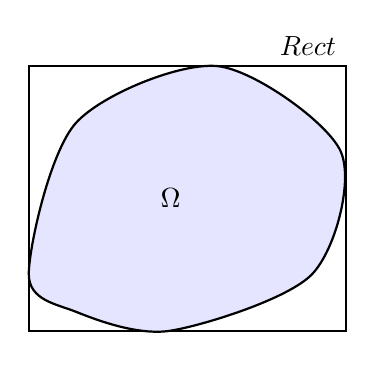
\begin{tikzpicture}[scale=1.2, thick]

% Rectangle (bounding box)
\draw[black] (1.5,0.6) rectangle (4.86,3.4);
\node[above left] at (4.86,3.4) {$\text{Rect}$};

% Generic domain inside (irregular blob)
\draw[fill=blue!10, thick, smooth cycle]
  plot coordinates {(1.5,1.2) (2,2.8) (3.5,3.4) (4.8,2.5)
                    (4.5,1.2) (3,0.6) (2,0.8)};

% Label for the inner domain
\node at (3,2) {$\Omega$};

% Optional: small arrows to suggest normal directions (decorative)
%\draw[->, gray!70] (6,2) -- +(0.5,0) node[right] {$n_R$};
%\draw[->, gray!70] (3.8,3.4) -- +(0,0.5) node[above] {$n_\Omega$};

\end{tikzpicture}
\caption{Rectangle circumscribing our domain $\Omega$.}
\label{fig:Omega}
\end{figure}
\\
The 
\begin{equation}
    \phi_{n,m} = \sqrt{\frac{2}{L_x}} \sin\left(\frac{\pi}{L_x} n x\right) \sqrt{\frac{2}{L_y}} \sin\left(\frac{\pi}{L_y} m y\right)
\end{equation}
are an orthonormal basis:
\begin{equation}
    \int_{\text{Rect}}dx\, \phi_{n,m}(x) \phi_{h, k}(x) = \delta_{n, h}\delta_{m, h},
\end{equation}
that is we can expand any function $\psi(x)$ as 
\begin{equation}
    \psi(x) = \sum_{n, m} c_{n, m}\phi_{n,m}.
\end{equation}
Let us now change the notation so to simplify it: instead of using two indices $n,m$ from $1$ to $N$, we will use a single index $i$ from $1$ to $M = N^2$. 
The expansion of $\psi$ then reads
\begin{equation}
    \psi(x) = \sum_i c_i \phi_i(x).
    \label{eq:em_psi}
\end{equation}
Suppose now $\psi(x)$ satisfies the Schrödinger equation over the domain $\Omega$
\begin{equation}
    H \psi = E \psi, 
\end{equation}
where the Hamiltonian $H$ is the Laplacian plus the potential
\begin{equation}
    V(x) = \begin{cases}
        0,& x \in \Omega \\
        \infty,& \text{otherwise}.
    \end{cases}
\end{equation}
It is useful in this problem to slightly change the potential in the following way
\begin{equation}
    V(x) = \begin{cases}
        0,& x \in \Omega \\
        V_0 (\gg \max\{E_n\}),& x \in \text{Rect} \setminus \Omega\\
        \infty,& \text{otherwise}.
    \end{cases}
\end{equation}
The region $\text{Rect} \setminus \Omega$ will also be called region II.\\
Substituting \eqref{eq:em_psi} we get 
\begin{equation}
    \sum_{ij} \left(H_{ij} - E \delta_{ij}\right) c_j = 0,
\end{equation}
where
\begin{equation}
    H_{ij} = \int_{\text{Rect}}dx\, \phi_{i}(x) H \phi_{j}(x) = E_{ij} \delta_{ij} + V_0 v_{ij},
\end{equation}
and 
\begin{equation}
    v_{ij} = \int_{\text{II}}dx\, \phi_{i}(x) \phi_{j}(x).
\end{equation}
So now the problem is to diagonalize the Hamiltonian.

\section{Results for the Stadium}
Let us consider a Bunimovich stadium, where the rectangle has length $L_x = 1, L_y = 2$. Consider, using our previous notation, different values $M = N^2 \in {1600, 2500, 3600, 4900}$, then solving the problem for the first $k = M/2$ eigenvalues
we obtain Fig.~\ref{fig:stadium_ene}.
\begin{figure}[h]
    \centering
    \includegraphics[width=0.5\textwidth]{../figs/stadium_eigenvalues_compare.png}
    \caption{Numerical energies for the Bunimovich stadium on the right, relative error $\frac{|E_i - E_{i -1}|}{E_{i-1}}$ for the energies on the left.}
    \label{fig:stadium_ene}
\end{figure}

\section{Unfolding the spectrum}
The chaotic properties of a quantum system lie in its spectrum, however, because the system is quantum, the lowest energetical levels are distant from each other, while the highest are next to each other.
This mean that before analyzing the spectrum, we have to perform a procedure, called \textit{unfolding}, which normalizes our spectrum into one with 
constant energy density $\rho$.
\\
We can unfold the spectrum using the Weyl's law \cite{B_cker_2011,Haake1991}, which states that the average number of states $N(E)$ up to the energy $E$, in the $2D$ case, are given by
\begin{equation}
    N_{avg}(E) = \frac{A}{4 \pi} E - \frac{L}{4 \pi} \sqrt{E} + C,
\end{equation}
where $A$ is the area of the billiard, $L$ is its perimeter and $C$ is a constant.
\\
We can now use this function to construct an unfolded spectrum $\epsilon$ where
\begin{equation}
    \epsilon_n = N_{avg}(E_n)
\end{equation}
and calculate the spacings $s$ of this spectrum
\begin{equation}
    s_n = \epsilon_{n + 1} - \epsilon_n.
\end{equation}
The chaotic properties then can be seen looking at the distribution of these spacings.
In particular we want to compare (Fig.~\ref{fig:pdf_comp})this histogram to two distributions: the Poisson 
\begin{equation}
    P(s) = e^{-s},
\end{equation}
which is the theoretical distribution for integrable system, and the GOE distribution
\begin{equation}
    P(s) = \frac{\pi s}{2} e^{-\pi s^2 / 4},
\end{equation}
which is the theoretical distribution for chaotic systems.
\begin{figure}[h]
    \centering
    \includegraphics[width=0.7\textwidth]{../figs/hist_ene_stadium_N1800.png}
    \caption{Plot of the histogram of out spacings and the two distributions defined previously. In this case we have computed $k = 1800$ eigenvalues.}
    \label{fig:pdf_comp}
\end{figure}

\clearpage
\bibliography{refs.bib}{}
\bibliographystyle{ieeetr}
\end{document}